% Chapter Template

\chapter{Désynchronisation de tâches} % Main chapter title

\label{Chapitre 2} % Change X to a consecutive number; for referencing this chapter elsewhere, use \ref{ChapterX}

\lhead{ \emph{Désynchronisation de tâches}} % Change X to a consecutive number; this is for the header on each page - perhaps a shortened title

Ce permier chapitre permet de montrer les différentes manières possibles de désynchroniser des tâches afin de les rendre moins gourmandes en ressources et plus performantes. 

%----------------------------------------------------------------------------------------
%	SECTION 1
%----------------------------------------------------------------------------------------
\section{Exemple d'application}

Nous aimerions bien avoir un petit compteur qui affiche le nombre de centième de seconde écoulé. L'affichage se fait à l'aide d'un afficheur 7 segments connecté sur les GPIOs du processeur et sur la FPGA. De plus, le compteur est contrôlé à l'aide de boutons poussoirs aussi connectés sur les différents GPIOs.
%-----------------------------------
%	SUBSECTION 2
%-----------------------------------
\subsection{Utilisation massive inutile du CPU}
Voici un premier bout code proposé qui fonctionne bien, mais qui est très mal optimisé :
\begin{lstlisting}[frame=single,style=C]  % Start your code-block

int main()
{
	int fd;
	fd=open("/dev/mem", O_RDWR);
	if(fd<0) {printf("Could not open /dev/mem: error=%i\n", fd); return fd;}
	gpio = mmap(0, 256, PROT_READ | PROT_WRITE, MAP_SHARED, fd, 0xd6000000);
	if(gpio==(void *)0xFFFFFFFF){printf("mmap failed, error: %i:%s \n",errno,strerror(errno)); return(-1);}
	while(1){
		for (int i=0; i<100; i++) {
			for (int j=0; j<10000; j++)
				seg7_display (i);
		}	
	}
	return 0;
}
\end{lstlisting}

Si on lance cette application et que l'on veut regarder sa consommation CPU :

\begin{lstlisting}[frame=single,style=Console]
$ top
\end{lstlisting}
\pagebreak Et voilà le résultat :


\begin{center} 
\hspace{12.45cm}
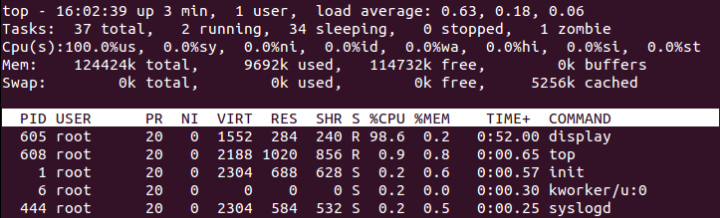
\includegraphics[width=12cm]{CPU_Bouffe.png}
\end{center}
\vspace{1cm}

On voit aisément que le CPU est utilisé à 98.8\%! Ce qui est  inacceptable sur un système embraqué limité en ressources pour toutes ses taches.

Pour contrer à ce problème, on peut utiliser les techniques suivantes :
\begin{enumerate}
\item Utiliser des timers
\item Utiliser des threads
\item Utilisation d'IPC avec un FIFO
\end{enumerate}


%----------------------------------------------------------------------------------------
%	SECTION 2
%----------------------------------------------------------------------------------------
\section{Utilisation de timers}

Afin de contrer au problème précédent, nous allons utiliser des timers pour réveiller le programme à un intervalle donné. Voici le "main" de ce programme qui utilise un timer:

\begin{lstlisting}[frame=single,style=C]  % Start your code-block

int main()
{
	int fd;
	fd=open("/dev/mem", O_RDWR);
	if(fd<0) {printf("Could not open /dev/mem: error=%i\n", fd); return fd;}
	gpio = mmap(0, 256, PROT_READ | PROT_WRITE, MAP_SHARED, fd, 0xd6000000);
	if(gpio==(void *)0xFFFFFFFF){printf("mmap failed, error: %i:%s \n",errno,strerror(errno)); return(-1);}

	//init du handler de SIGALRM
	if(signal(SIGALRM, sigALRM_handler) == SIG_ERR)
	{
		perror("SIGALRM handler");
		exit(EXIT_FAILURE);
	}
	//création d'un itimer pour générer le SIGALRM
	struct itimerval aItimerval;
	aItimerval.it_interval.tv_sec = 0;
	aItimerval.it_interval.tv_usec = 10000;
	aItimerval.it_value.tv_sec = 0;
	aItimerval.it_value.tv_usec = 10000;
	if(setitimer(ITIMER_REAL, &aItimerval, NULL) < 0)
	{
		perror("setitimer");
		exit(EXIT_FAILURE);
	}
	//sleep du programme
	while(1)
	{
		safeSleep(100000000);
		gCounter++;
		if(gCounter==100)
			gCounter=0;
	}
	return 0;
}
\end{lstlisting}

La première chose que l'on fait c'est d'initialiser le "handler" qui va trigger sur le signal SIGALRM. Et évidemment pour cela, il faut lui passer la fonction qui va devoir être appelée.\\
 

On construit ensuite un "itimer" qui va lancer périodiquement les signaux SIGALRM (utilisé pour rafraîchir l'écran).
La boucle principale est simple : on endort le programme pendant environ 100ms pour ensuite incrémenter le compteur.\\


Le handler du "itimer" est très simple : il appelle uniquement la fonction de rafraîchissement. Voilà le code :

\begin{lstlisting}[frame=single,style=C]  % Start your code-block

//handler pour le signal SIGALRM pour rafraichir l'affichage 7 seg
static void sigALRM_handler(int signo)
{
	seg7_display (gCounter);
	
	return;
}
\end{lstlisting}


Nous utilisons la fonction "nanosleep" pour endormir la boucle principale. Cette fonction est "malheureusement" interruptible par les signaux SIGALRM.Donc il faut tester les valeurs de sorties!\\


Voilà l'implémentation de cette fonction.

 
\begin{lstlisting}[frame=single,style=C]  % Start your code-block

//sleep sécurisé pour le cas ou il est interrompu trop tot par
void safeSleep(int ns)
{
	int ret;
	struct timespec req, rem;
	req.tv_sec = 0;
	req.tv_nsec = ns;
	while(1)
	{
		ret = nanosleep(&req, &rem);
		if(ret)
		{
			if(errno == EINTR)
			{
				req.tv_sec = rem.tv_sec;
				req.tv_nsec = rem.tv_nsec;
			}
			else perror("nanosleep");
		}
		else return;
	}
}
\end{lstlisting}

\pagebreak Le résultat de ce nouveau programme (qui implémente exactement la même fonctionnalité que l'exemple précédent) est excellent. Voici sa consommation CPU :

\begin{center} 
\hspace{12.45cm}
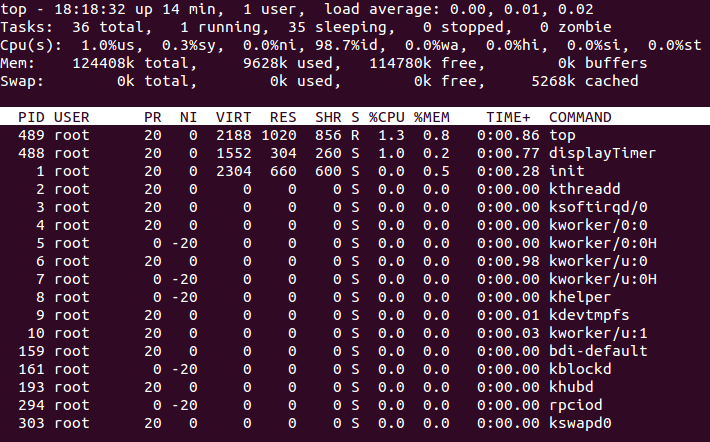
\includegraphics[width=12.5cm]{CPU_itimer.png}
\end{center}
\vspace{1cm}


On voit que cette fois la consommation CPU est passée de 98.8\% à 1.0\%! Donc notre technique est très concluante.

%----------------------------------------------------------------------------------------
%	SECTION 3
%----------------------------------------------------------------------------------------
\newpage\section{Utilisation de threads}
Au lieu d'utiliser des timers pour réveiller le programme à un intervalle donné, on utilise ici deux thread qui vont se réveiller périodiquement (ou plutôt s'endormir pendant un intervalle donné). Le partage des données se fait au travers d'une variable globale comme pour les autres exemples. 

L'idée est d'avoir :
\begin{itemize}
\item Un thread qui s'occupe du multiplexage des afficheurs
\item Un thread qui compte le temps (100ms)\\
\end{itemize}

Donc voilà rapidement le code que nous proposons :
 
\begin{lstlisting}[frame=single,style=C]  % Start your code-block

// Shared time var
static volatile int8_t gTimeValue = 0;

void thread_mux(void *pdata)
{
	uint8_t left = 0;

	while(1)
	{
		seg7_display (gTimeValue,left%2);
		usleep(2000);
		left+=1;
	}
}

void thread_sec(void *pdata)
{
	while(1)
	{
		gTimeValue= (++gTimeValue)%100;
		usleep(100000);
	}
}	

int main()
{
	pthread_t muxThread,secThread;
	int fd;
	void *ret1,*ret2;

	fd=open("/dev/mem", O_RDWR);
	if(fd<0) {printf("Could not open /dev/mem: error=%i\n", fd); return fd;}
	gpio = mmap(0, 256, PROT_READ | PROT_WRITE, MAP_SHARED, fd, 0xd6000000);
	if(gpio==(void *)0xFFFFFFFF){printf("mmap failed, error: %i:%s \n",errno,strerror(errno)); return(-1);}
	
	// Thread creation
	if(pthread_create(&muxThread,NULL,thread_mux,"Multiplexer Threads")<0)
	{
		perror("Multiplexer Thread");exit(-1);
	}

	// Thread creation
	if(pthread_create(&secThread,NULL,thread_sec,"Seconds Threads")<0)
	{
		perror("Seconds Thread");exit(-1);
	}
	(void) pthread_join(muxThread,&ret1);
	(void) pthread_join(secThread,&ret2);

	return 0;
}
\end{lstlisting}

\pagebreak Il n'y a pas beaucoup de commentaires à faire. Le code est très simple : la boucle principale instancie les 2 threads et attend  qu'il aient terminés. Les deux threads implémentent les fonctionnalités séparément.\\


Le résultat de cette implémentation est bien aussi, mais il est moins performant que le précédent. Il consomme un peu moins de 2\% de CPU.

 
%----------------------------------------------------------------------------------------
%	SECTION 4
%----------------------------------------------------------------------------------------
\newpage\section{Utilisation de FIFOs}
Nous voilà arrivé à une partie intéressante. LE but est cette fois de faire communiquer les processus (et non des threads) en utilisant des FIFOs. Comme sur Linux tout est fichier, un FIFO est aussi un fichier.\\
\subsection{FIFO en lecture}
L'idée ici est toujours d'utiliser un timer pour gérer le multiplexage des afficheurs, mais cette fois la commande pour incrémenter le compteur est passé par un FIFO (histoire de voir comment fonctionne la communication inter-processus).Voilà le code exemple :
\begin{lstlisting}[frame=single,style=C]  % Start your code-block

int main()
{
	// ....
	// FPGA ....
	// Initialisation du itimer
	// ....
	//création d'un FIFO
	int fd_mk_fifo;
	fd_mk_fifo = mkfifo(FIFO_NAME, 0666);

	if(fd_mk_fifo < 0)
	{
		perror("mkfifo");
		exit(EXIT_FAILURE);
	}
	//ouverture du FIFO en lecture
	int fd_open_fifo;
	fd_open_fifo = open(FIFO_NAME, O_RDONLY);
	if(fd_open_fifo <= 0)
	{
		perror("openFIFO");
		exit(EXIT_FAILURE);
	}

	while(1)
	{
		//lecture du FIFO
		char str_fifo[STR_FIFO_LENGTH];
		int n;
		//sleep pour économiser le temps processeur
		// car la fonction "read" s'est montrée non bloquante...
		safeSleep(10000000);

		n = read(fd_open_fifo, str_fifo, STR_FIFO_LENGTH);
		str_fifo[n]='\0';

		//analyse du contenu
		if(strcmp(str_fifo, "PLUS\n") == 0)
		{
			if(gCounter == 99)
				gCounter = 0;
			else gCounter++;
		}else if(strcmp(str_fifo, "MINUS\n") == 0)
		{
			if(gCounter == 0)
				gCounter = 99;
			else gCounter--;
		}else if(strcmp(str_fifo, "NULL\n") == 0)
		{
			gCounter = 0;
		}
	}
	return 0;
}
\end{lstlisting}

\newpage On peut voir que l'on crée le FIFO et ensuite qu'on lit celui-ci afin d'obtenir les commandes:
\begin{itemize}
\item "PLUS" : Pour ajouter un au compteur
\item "MINUS" : Pour soustraire un au compteur
\item "NULL" : Pour remettre le compteur à zéro\\
\end{itemize}

Comme pour l'exemple du "itimer" (sans FIFO), on utilise une variable globale pour communiquer avec le handler du timer.\\

Voilà le résultat obtenu :
\begin{center} 
\hspace{12.45cm}
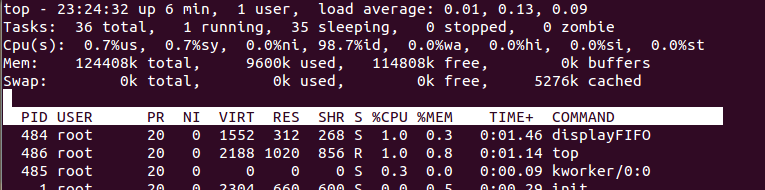
\includegraphics[width=12.5cm]{CPU_FIFODisplay.png}
\end{center}
\vspace{1cm}

Donc on voit que cette solution est aussi performante que la première. Seulement 1\% de consommation CPU.\\\\

\textbf{Remarques : la fonction "read" du FIFO n'était pas bloquante, d'ou l'utilisation d'un timer ! Nous n'avons pas compris pourquoi la fonction "read" n'était pas bloquante.}

\newpage\subsection{FIFO en écriture}
Ce qui serait intéressant maintenant, c'est de créer un second processus qui interagit avec le FIFO créé. Pour cela, nous avons utilisé un programme exemple qui lit les boutons connectés aux GPIOs. Nous l'avons adapté pour utiliser le FIFO et dans ce cas modifier directement le compteur.Voilà le code de ce programme:

\begin{lstlisting}[frame=single,style=C]  % Start your code-block

int main()
{
	//.....
	// Stuff initialization
	// .....
	//ouverture du FIFO en lecture
	int fd_open_fifo;
	fd_open_fifo = open(FIFO_NAME, O_WRONLY);
	if(fd_open_fifo <= 0)
	{
		perror("openFIFO");
		exit(EXIT_FAILURE);
	}
	//variables des boutons
	int bt_plus, bt_moins, bt_null;
	
	while (1)
	{
		button_state = ~(gpio->leds_rw >> 8) & 0x7;
		//printf("result =0x%02x\n", button_state);
		usleep(500000);

		bt_plus = button_state & 0x01;
		bt_moins = button_state & 0x02;
		bt_null = button_state & 0x04;

		//écriture dans le FIFO
		if(bt_plus)
		{
			if(write(fd_open_fifo, "PLUS\n", 5) != 5)
			{
			perror("write"); 
			}
		}
		else if(bt_moins)
		{
			if(write(fd_open_fifo, "MINUS\n", 6) != 6)
			{
			perror("write"); 
			}
		}
		else if(bt_null)
		{
			if(write(fd_open_fifo, "NULL\n", 5) != 5)
			{
			perror("write"); 
			}
		}
	}
	munmap ((void*)gpio, 256);
	close (fd);
	return 0;
}
\end{lstlisting}

\pagebreak C'est très simple, on ouvre le fichier FIFO en écriture et on teste en boucle les boutons poussoir. Selon leurs états, on va écrire les différente commandes ("PLUS","MINUS" ou "NULL") dans le FIFO. Ce qui va faire changer la valeur du compteur.\\

Voilà le résultat de ce test final :

\begin{center} 
\hspace{12.45cm}
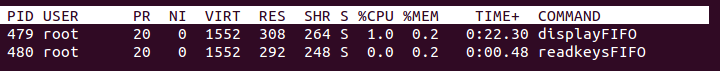
\includegraphics[width=12.5cm]{CPU_FIFOFull.png}
\end{center}
\vspace{1cm}


 


